\documentclass{standalone}

\usepackage{tikz, tikz-3dplot} % for 2D and 3D graphics

\definecolor{ocre}{RGB}{0,83,166}

\begin{document}

\tdplotsetmaincoords{75}{135}
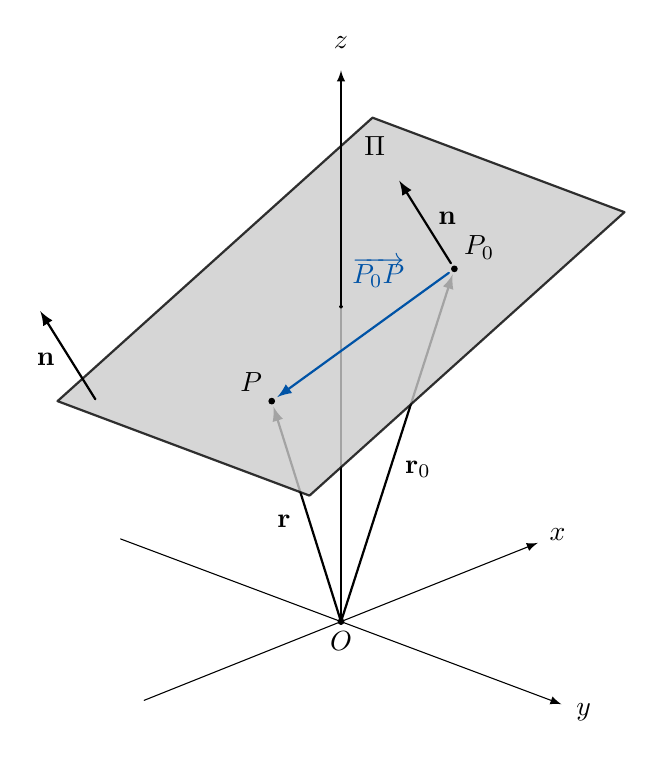
\begin{tikzpicture}[x={(1cm,0.4cm)}, y={(8mm, -3mm)}, z={(0cm,1cm)}, line cap=round, line join=round]
    %Coordinates
        %Plane Vertex Points
    \coordinate (x1) at (-2,2,3);
    \coordinate (x2) at (2,2,5);
    \coordinate (x3) at (2,-2,5);
    \coordinate (x4) at (-2,-2,3);
    %Vectors Parallel to Plane
    \coordinate (n1) at ($(x2) - (x1)$);
    \coordinate (n2) at ($(x2) - (x3)$); 
    %Points on Plane
    \coordinate (x5) at ($(x1) + 0.04*(n1) - 0.9*(n2)$);
    \node[outer sep = 1pt, inner sep = 1pt] (x6) at ($(x1) + 0.7*(n1) - 0.3*(n2)$) {};
    \coordinate (x7) at ($(x1) + 0.5*(n1) - 0.5*(n2)$);
    %Beginning of Axis
    \coordinate (O) at (0,0,0);
    %Random Point
    \node[outer sep = 1pt, inner sep = 1pt] (P) at ($(x1) + 0.2*(n1) - 0.4*(n2)$) {};
    
        %Axis     
    \draw[-latex] (-2.5,0,0) -- (2.5,0,0) node[pos = 1.05] {$x$};
    \draw[-latex] (0,-3.5,0) -- (0,3.5,0) node[pos = 1.05] {$y$};
    \draw[-latex] (0,0,0) -- (0,0,7) node[pos = 1.05] {$z$};
    \draw[draw=black, fill=black] (O) circle (1pt) node[below] {${O}$};
    
        %Point on Plane
    \draw[-latex, thick] (O) -- (x6) node[pos=0.45, shift={(0.1,0.3)}] {$\mathbf{r}_0$};
    \draw[-latex, thick] (O) -- (P) node[pos=0.45, shift={(-0.1,-0.3)}] {$\mathbf{r}$};
    %Plane
        \path[draw=black, fill=black!20, thick, opacity = 0.8] (x1) -- (x2) -- (x3) -- (x4) -- (x1);
    \node[shift={(-0.45,0.6)}] at (x3) {$\Pi$};
    %Perpendicular Vector
    \coordinate (direction_vec) at ($(-8,0,16) - (x5)$);

    % Perpendicular Vector at x5
    \draw[-latex, thick] (x5) -- ($(x5) - 0.7*(1,0,-2)$) node[pos=0.5, shift={(-0.2,-0.1)}] {$\mathbf{n}$};
    
    % Parallel Vector at x6
    % Now add the scaled vector to x6
    \draw[-latex, thick] (x6) -- ($(x6) - 0.7*(1,0,-2)$) node[pos=0.5, shift={(0.2,0.1)}] {$\mathbf{n}$};
    
        %Point on Plane    
    \draw[draw=black, fill=black] (x6) circle (1pt) node[above right] {${P}_0$};
    
        %Z-axis Section
    \draw[draw=black, fill=black] (x7) circle (0.5pt);
    \draw (x7) -- (0,0,6.5);
    
        %Random Point
    \draw[draw=black, fill=black] (P) circle (1pt) node[above left] {$P$};
    \draw[-latex, thick, ocre] (x6) -- (P) node[pos=0.2, above left] {$\overrightarrow{P_0P}$};
\end{tikzpicture}

\end{document}